%!TEX encoding = UTF-8 Unicode
%!TEX root = ../lect-w10.tex

%%%

\ifkompendium\else


\Subsection{Grupplaboration}



\begin{Slide}{Grupplaboration: \texttt{snake} över 2 veckor}
\begin{minipage}{0.6\textwidth}
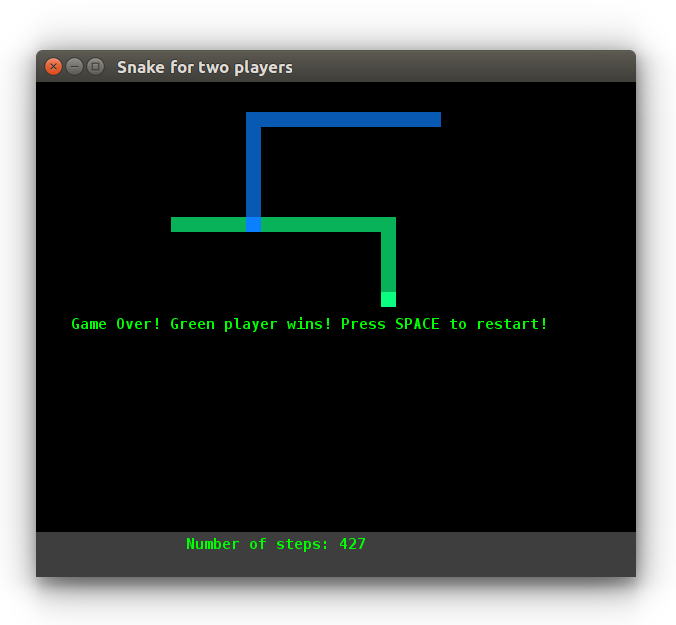
\includegraphics[width=1.0\textwidth]{../img/snake-twoplayer}
\end{minipage}%
\begin{minipage}{0.4\textwidth}
\begin{itemize}
%!TEX encoding = UTF-8 Unicode
%!TEX root = ../compendium2.tex

\item Kunna använda arv.
\item Kunna göra överskuggning av medlemmar i en supertyp.
%\item Kunna referera till medlemmar i superklassen med \code{super} vid överskuggning.
\item Kunna förklara begreppet dynamisk bindning.
\item Kunna använda abstrakta klasser och skapa en klasshierarki.

\end{itemize}
\end{minipage}%
\end{Slide}

\begin{Slide}{Arvshierarki i \texttt{snake}: Olika typer av varelser}
  \begin{center}
  \newcommand{\TextBox}[1]{\raisebox{0pt}[1em][0.5em]{#1}}
  \tikzstyle{umlclass}=[rectangle, draw=black,  thick, anchor=north, text width=2.5cm, rectangle split, rectangle split parts = 3]
  \begin{tikzpicture}[inner sep=0.5em,scale=0.8, every node/.style={transform shape}]

    \node [umlclass, rectangle split parts = 1, xshift=-1.0cm, yshift=4.5cm] (BaseType)  {
                \textit{\textbf{\centerline{\TextBox{\code{Entity}}}}}
  %              \nodepart[align=left]{second}\code{def x: T} \newline \code{def y: T}
            };


    \node [umlclass, rectangle split parts = 1, xshift=-3cm, yshift=2.5cm] (SubType1)  {
                \textit{\textbf{\centerline{\TextBox{\code{CanMove}}}}}
  %              \nodepart[align=left]{second}\code{val x: Int} \newline \code{val y: Int}
            };

  \node [umlclass, rectangle split parts = 1, xshift=-4.5cm, yshift=0.5cm] (SubSubType0)  {
              {\textbf{\centerline{\TextBox{\code{Snake}}}}}
  %            \nodepart[]{second}\TextBox{\code{val dim: Int}}
  };


  \node [umlclass, rectangle split parts = 1, xshift=0.75cm, yshift=2.5cm] (SubType2)  {
              \textit{\textbf{\centerline{\TextBox{\code{CanTeleport}}}}}
  %            \nodepart[]{second}\TextBox{\code{val dim: Int}}
          };

  \node [umlclass, rectangle split parts = 1, xshift=-1.0cm, yshift=0.5cm] (SubSubType1)  {
              {\textbf{\centerline{\TextBox{\code{Apple}}}}}
  %            \nodepart[]{second}\TextBox{\code{val dim: Int}}
          };

  \node [umlclass, rectangle split parts = 1, xshift=2.5cm, yshift=0.5cm] (SubSubType2)  {
              {\textbf{\centerline{\TextBox{\code{Banana}}}}}
  %            \nodepart[]{second}\TextBox{\code{val dim: Int}}
          };


  \draw[umlarrow] (SubType1.north) -- ++(0,0.5) -| (BaseType.south);
  \draw[umlarrow] (SubType2.north) -- ++(0,0.5) -| (BaseType.south);
  \draw[umlarrow] (SubSubType1.north) -- ++(0,0.5) -| (SubType2.south);
  \draw[umlarrow] (SubSubType2.north) -- ++(0,0.5) -| (SubType2.south);
  \draw[umlarrow] (SubSubType0.north) -- ++(0,0.5) -| (SubType1.south);

  \end{tikzpicture}
  \end{center}
\end{Slide}


\begin{Slide}{Arvshierarki i \texttt{snake}: Olika typer av spel}
  \begin{center}
  \newcommand{\TextBox}[1]{\raisebox{0pt}[1em][0.5em]{#1}}
  \tikzstyle{umlclass}=[rectangle, draw=black,  thick, anchor=north, text width=3cm, rectangle split, rectangle split parts = 3]
  \begin{tikzpicture}[inner sep=0.5em,scale=0.8, every node/.style={transform shape}]

    \node [umlclass, rectangle split parts = 1, xshift=0cm, yshift=5cm] (BaseType)  {
                \textit{\textbf{\centerline{\TextBox{\code{BlockGame}}}}}
  %              \nodepart[align=left]{second}\code{def x: T} \newline \code{def y: T}
            };


    \node [umlclass, rectangle split parts = 1, xshift=0cm, yshift=3.0cm] (SubType)  {
                \textit{\textbf{\centerline{\TextBox{\code{SnakeGame}}}}}
  %              \nodepart[align=left]{second}\code{val x: Int} \newline \code{val y: Int}
            };

  \node [umlclass, rectangle split parts = 1, xshift=-3cm, yshift=0.5cm] (SubSubType1)  {
              {\textbf{\centerline{\TextBox{\code{OnePlayerGame}}}}}
  %            \nodepart[]{second}\TextBox{\code{val dim: Int}}
          };

  \node [umlclass, rectangle split parts = 1, xshift=3cm, yshift=0.5cm] (SubSubType2)  {
              {\textbf{\centerline{\TextBox{\code{TwoPlayerGame}}}}}
  %            \nodepart[]{second}\TextBox{\code{val dim: Int}}
          };

  \draw[umlarrow] (SubType.north) -- ++(0,0.5) -| (BaseType.south);
  \draw[umlarrow] (SubSubType1.north) -- ++(0,0.5) -| (SubType.south);
  \draw[umlarrow] (SubSubType2.north) -- ++(0,0.5) -| (SubType.south);

  \end{tikzpicture}
  \end{center}
\end{Slide}

\begin{Slide}{Krav vid respektive gruppstorlek}
Krav som minst ska implementeras vid olika gruppstorlek:

\vspace{1em}
  \begin{tabular}{r | c c c c c c}
    \Alert{Krav} / \Emph{Antal personer} & 1       & 2       & 3       & 4       & 5       & 6 \\ \hline
    \texttt{Player}       & $\surd$ & $\surd$ & $\surd$ & $\surd$ & $\surd$ & $\surd$ \\
    \texttt{OnePlayerGame}& $\surd$ &         &         &         & $\surd$ & $\surd$ \\
    \texttt{TwoPlayerGame}&         & $\surd$ & $\surd$ & $\surd$ & $\surd$ & $\surd$ \\
    \texttt{Snake}        & $\surd$ & $\surd$ & $\surd$ & $\surd$ & $\surd$ & $\surd$ \\
    \texttt{Apple}        & $\surd$ &         & $\surd$ & $\surd$ & $\surd$ & $\surd$ \\
    \texttt{Banana}       &         &         &         & $\surd$ &         & $\surd$ \\
  \end{tabular}

\vspace{1em}
\begin{itemize}\SlideFontSmall
\item Uppgiften lämpar sig bäst för minst 3 gruppmedlemmar. 
\item Prata med handledare: slå ihop två små grupper till en med max 6 st.
\item Om du har särskilda skäl, t.ex. många restlabbar, kan du efter godkännande från kursansvarig göra labben enskilt.

\end{itemize}
\end{Slide}


\begin{Slide}{Instruktioner Grupplaboration}
\begin{itemize}\SlideFontSmall
%!TEX encoding = UTF-8 Unicode
%!TEX root = compendium.tex
\item 
Diskutera i din samarbetsgrupp hur ni ska dela upp koden mellan er i flera olika delar, som ni kan arbeta med var för sig. En sådan del kan vara en klass, en trait, ett objekt, ett paket, eller en funktion. 
\item
Varje del ska ha en \emph{huvudansvarig} individ. 
\item
Arbetsfördelningen ska vara någorlunda jämnt fördelad mellan gruppmedlemmarna.
\item
När ni redovisar er lösning ska ni börja med att redogöra för handledaren hur ni delat upp koden och vem som är huvudansvarig för vad. 
\item
Den som är huvudansvarig för en viss del redovisar den delen.
\item 
Grupplaborationer görs i huvudsak som hemuppgift. Salstiden används primärt för redovisning.
\end{itemize}
\end{Slide}

%!TEX encoding = UTF-8 Unicode
%!TEX root = ../lect-w09.tex

\begin{Slide}{Kodgranskning under grupplaborationen \texttt{snake}}
Grupplaborationen \code{snake} går över två läsveckor (w10--w11). Du ska:
\begin{itemize}
\item delta i framtagande av en gemensam checklista för kodgranskning,
\item granska minst en annan gruppmedlems kod,
\item bjuda in minst en annan gruppmedlem att granska din kod,
\item ge konstruktiv feedback,
\item ta emot konstruktiv feedback och försöka förbättra din kod,
\item på redovisning redogöra för nyttan och utmaningarna med kodgranskningar utifrån dina egna erfarenheter.
\end{itemize}
Mer om kodgranskning i efterföljande kurser, t.ex. ''Programvaruutveckling i grupp'' och ''Programvaruutveckling för stora system''
\end{Slide}


\begin{Slide}{Redovisning på obligatorisk schemalagd labbtid}
Första \code{snake}-veckan (w10):
\begin{itemize}\SlideFontTiny
\item Redovisa uppdelning av uppgiften mellan gruppmedlemmar och hur långt du har kommit med din del. Visa en skriftlig plan för implementationsarbetet för andra veckan, med valda deluppgifter och sluttidpunkter.
\item Redovisa arbetet med granskningar, minst checklista och planering för arbetet med granskningar i andra veckan. Bra om ni du gjort någon granskning.
\item Jobba vidare med \code{snake} och få hjälp av handledare om du kör fast. 
\end{itemize}
Andra \code{snake}-veckan (w11):
\begin{itemize}\SlideFontTiny
\item Redogör för uppdelningen av uppgiften och avgränsningen av ditt huvudansvar.
\item Förklara övergripande hela kodbasens struktur och syftet med de olika kod-delarna.
\item Förklara mer ingående de delar där du bidragit till implementationen.
\item Gör en kort demonstration av det körande systemet och visa vilka valfria uppgifter ni valt att göra.
\item Beskriv utmaningar med systemutveckling i grupp utifrån dina egna erfarenheter.
\item Redogör för nyttan och utmaningarna med kodgranskningar utifrån dina egna erfarenheter.  
\end{itemize}
\end{Slide}

\begin{Slide}{Övning w10: \texttt{inheritance}}
\begin{itemize}\SlideFontTiny
%!TEX encoding = UTF-8 Unicode

%!TEX root = ../compendium2.tex

\item Kunna deklarera och använda en arvshierarki i flera nivåer med nyckelordet \code{extends}.

\item Känna till synlighetsregler vid arv och nyttan med privata och skyddade medlemmar och nyckelorden \code{private} och \code{protected}.

%\item Kunna deklarera och använda skyddade medlemmar.

\item Kunna deklarera och använda överskuggade medlemmar och nyckelordet \code{override}.

\item Kunna deklarera och använda en hierarki av klasser där konstruktorparametrar överförs till superklasser.

\item Kunna deklarera och använda uppräknade värden med case-objekt och gemensam bastyp.

\item Känna till reglerna som gäller vid överskuggning av olika sorters medlemmar.

\item Känna till nyttan med finala klasser och finala attribut och nyckelordet \code{final}.

\item Kännedom om dessa begrepp:
bastyp,
sypertyp,
subtyp,
körtidstyp,
dynamisk bindning,
polymorfism,
trait,
inmixning,
överskuggad medlem,
anonym klass,
skyddad medlem,
abstrakt medlem,
abstrakt klass,
referenstyp,
värdetyp.



%TODO KOLLA PÅ NEDAN MÅL OCH BESTÄM HUR DE SKA IN I ÖVNINGARNA

%\item Känna till hur typtester och typkonvertering under körtid kan göras med metoderna \code{isInstanceOf} och \code{asInstanceOf} och känna till att detta görs bättre med \code{match}.

%\item Kunna deklarera och använda inmixning med flera traits och nyckelordet \code{with}.

%\item Kunna referera till medlem i superklassen med referensen \code{super} och känna till när detta nyckel ord behövs.

%\item Känna till begreppet anonym klass.

\end{itemize}
\end{Slide}

% \begin{Slide}{Extraundervisning del 2}
% För de som har det extra svårt, på samma sätt som förra ons:
% \begin{itemize}
% \item  \Alert{Extraundervisning} i \Emph{E:3308} onsdag 14/11 kl 15:15-17:00
% \item Hitta dit: \url{http://fileadmin.cs.lth.se/ehus/E3308.pdf}
% \item Det finns gott om platser i den salen men om fullt så förtur för de med kontrollskrivningspoäng < 15
% \item Fokus: grundläggande, långsam behandling på begäran av viktigaste koncepten från lp1
% \item Förberedelse: kolla på din kontrollskrivning del B och välj ut något specifikt som du vill ha hjälp med att förstå. \\ Kolla ks här: \url{http://cs.lth.se/pgk/examination/}
% \end{itemize}
% \end{Slide}


\begin{Slide}{Gästföreläsning: Kodgranskningar}
Hjärtligt välkommen: \\ \Emph{Gustaf Lundh}, Senior Developer, Axis
\end{Slide}

\fi
